\documentclass[12pt]{article}
\usepackage[utf8]{inputenc}
\usepackage[T1]{fontenc}
\usepackage[polish]{babel}
\usepackage{geometry}
\usepackage{tabularx}
\usepackage[table,xcdraw,dvipsnames]{xcolor}
\usepackage{color}
\usepackage{subfig}
\usepackage{sidecap}
\usepackage{wrapfig}
\usepackage{float}
\usepackage{enumerate}
\usepackage{graphicx}
\usepackage{multirow}
\usepackage{hyperref}
\usepackage{titlesec}
\usepackage{amsmath}
\usepackage{anyfontsize}
\usepackage{indentfirst}
\usepackage{listings}
\usepackage{multicol}
\usepackage{pgfplots}
\usepackage{fancyhdr}

\newgeometry{tmargin=1.8cm,bmargin=1.8cm,lmargin =1.8cm,rmargin=1.8cm}
\begin{document}

\begin{titlepage}
\begin{figure}
    \centering
    
\includegraphics[width=18cm]{logo-PWr.png}
    \label{fig:pwr}
\end{figure}
    \begin{center}
        \LARGE \textbf{ Wydział Elektroniki, Fotoniki i Mikrosystemów }\\ 
        \vspace{70pt}
        \Huge \textit{ Sterowanie Procesami Ciągłymi}  \\
    \end{center}
    \vspace{30pt}
    \hrule
    \vspace{1pt}
    \hrule
    \begin{center}
        {\fontsize{30}{50}\selectfont Sprawozdanie nr 1\\ }
        \vspace{10pt}
        {\fontsize{25}{25}\selectfont Charakterystyki czasowe  }
    \end{center}
    \hrule
    \vspace{1pt}
    \hrule
    \begin{flushright}
        \vspace{50pt}

        \textit{\Large Prowadzący:}\\
        \Large dr hab. inż. Grzegorz Mzyk\\
        \vspace{10pt}
        \textit{\Large Wykonała:}\\
        \Large Zuzanna Mejer, 259382 \\
        \vspace{10pt}
        \textit{\Large Termin zajęć:}\\
        \Large czwartek TP, 9:15\\
        \vspace{10pt}
    
    \end{flushright}
    \vspace{60pt}
    \begin{center}
        \large Wrocław, \today r.
    \end{center}
\end{titlepage}
    
    
\tableofcontents
\newpage

\section{Cel ćwiczenia}
Celem ćwiczenia jest zapoznanie się z charakterystykami czasowymi systemów. Ćwiczenie można podzielić na dwie części - zapoznanie się z zależnością charakterystyki skokowej od położenia biegunów transmitancji układów oraz próba identyfikacji systemów z czasem ciągłym na podstawie charakterystyk skokowych.


\section{Badanie systemów z czasem ciągłym}

Rozpatrywany jest system ciągły o transmitancji w postaci:
\begin{equation}
    K(s) = \frac{1}{s^2+as+b},
\end{equation}
którą można przedstawić również jako:
\begin{equation}
    K(s) = \frac{1}{(s+b_1)(s+b_2)},
\end{equation}
gdzie $b_1$ oraz $b_2$ to bieguny. W zależności od ich położenia badano odpowiedź skokową układu.

\subsection{Położenie biegunów a odpowiedź skokowa układu}

\subsubsection{Bieguny rzeczywiste, ujemne}
Przyjmując wartości biegunów:
\begin{equation*}
    \left\{{{b_1 = -3}\atop {b_2 = -2}}\right.
\end{equation*}

Transmitancja systemu to:
\begin{equation}
    K(s) = \frac{1}{(s-(-3))(s-(-2))} = \frac{1}{(s+3)(s+2)} = \frac{1}{s^2+5s+6}
\end{equation}

Wygenerowano odpowiedź skokową systemu:

\begin{figure}[H]
    \centering
    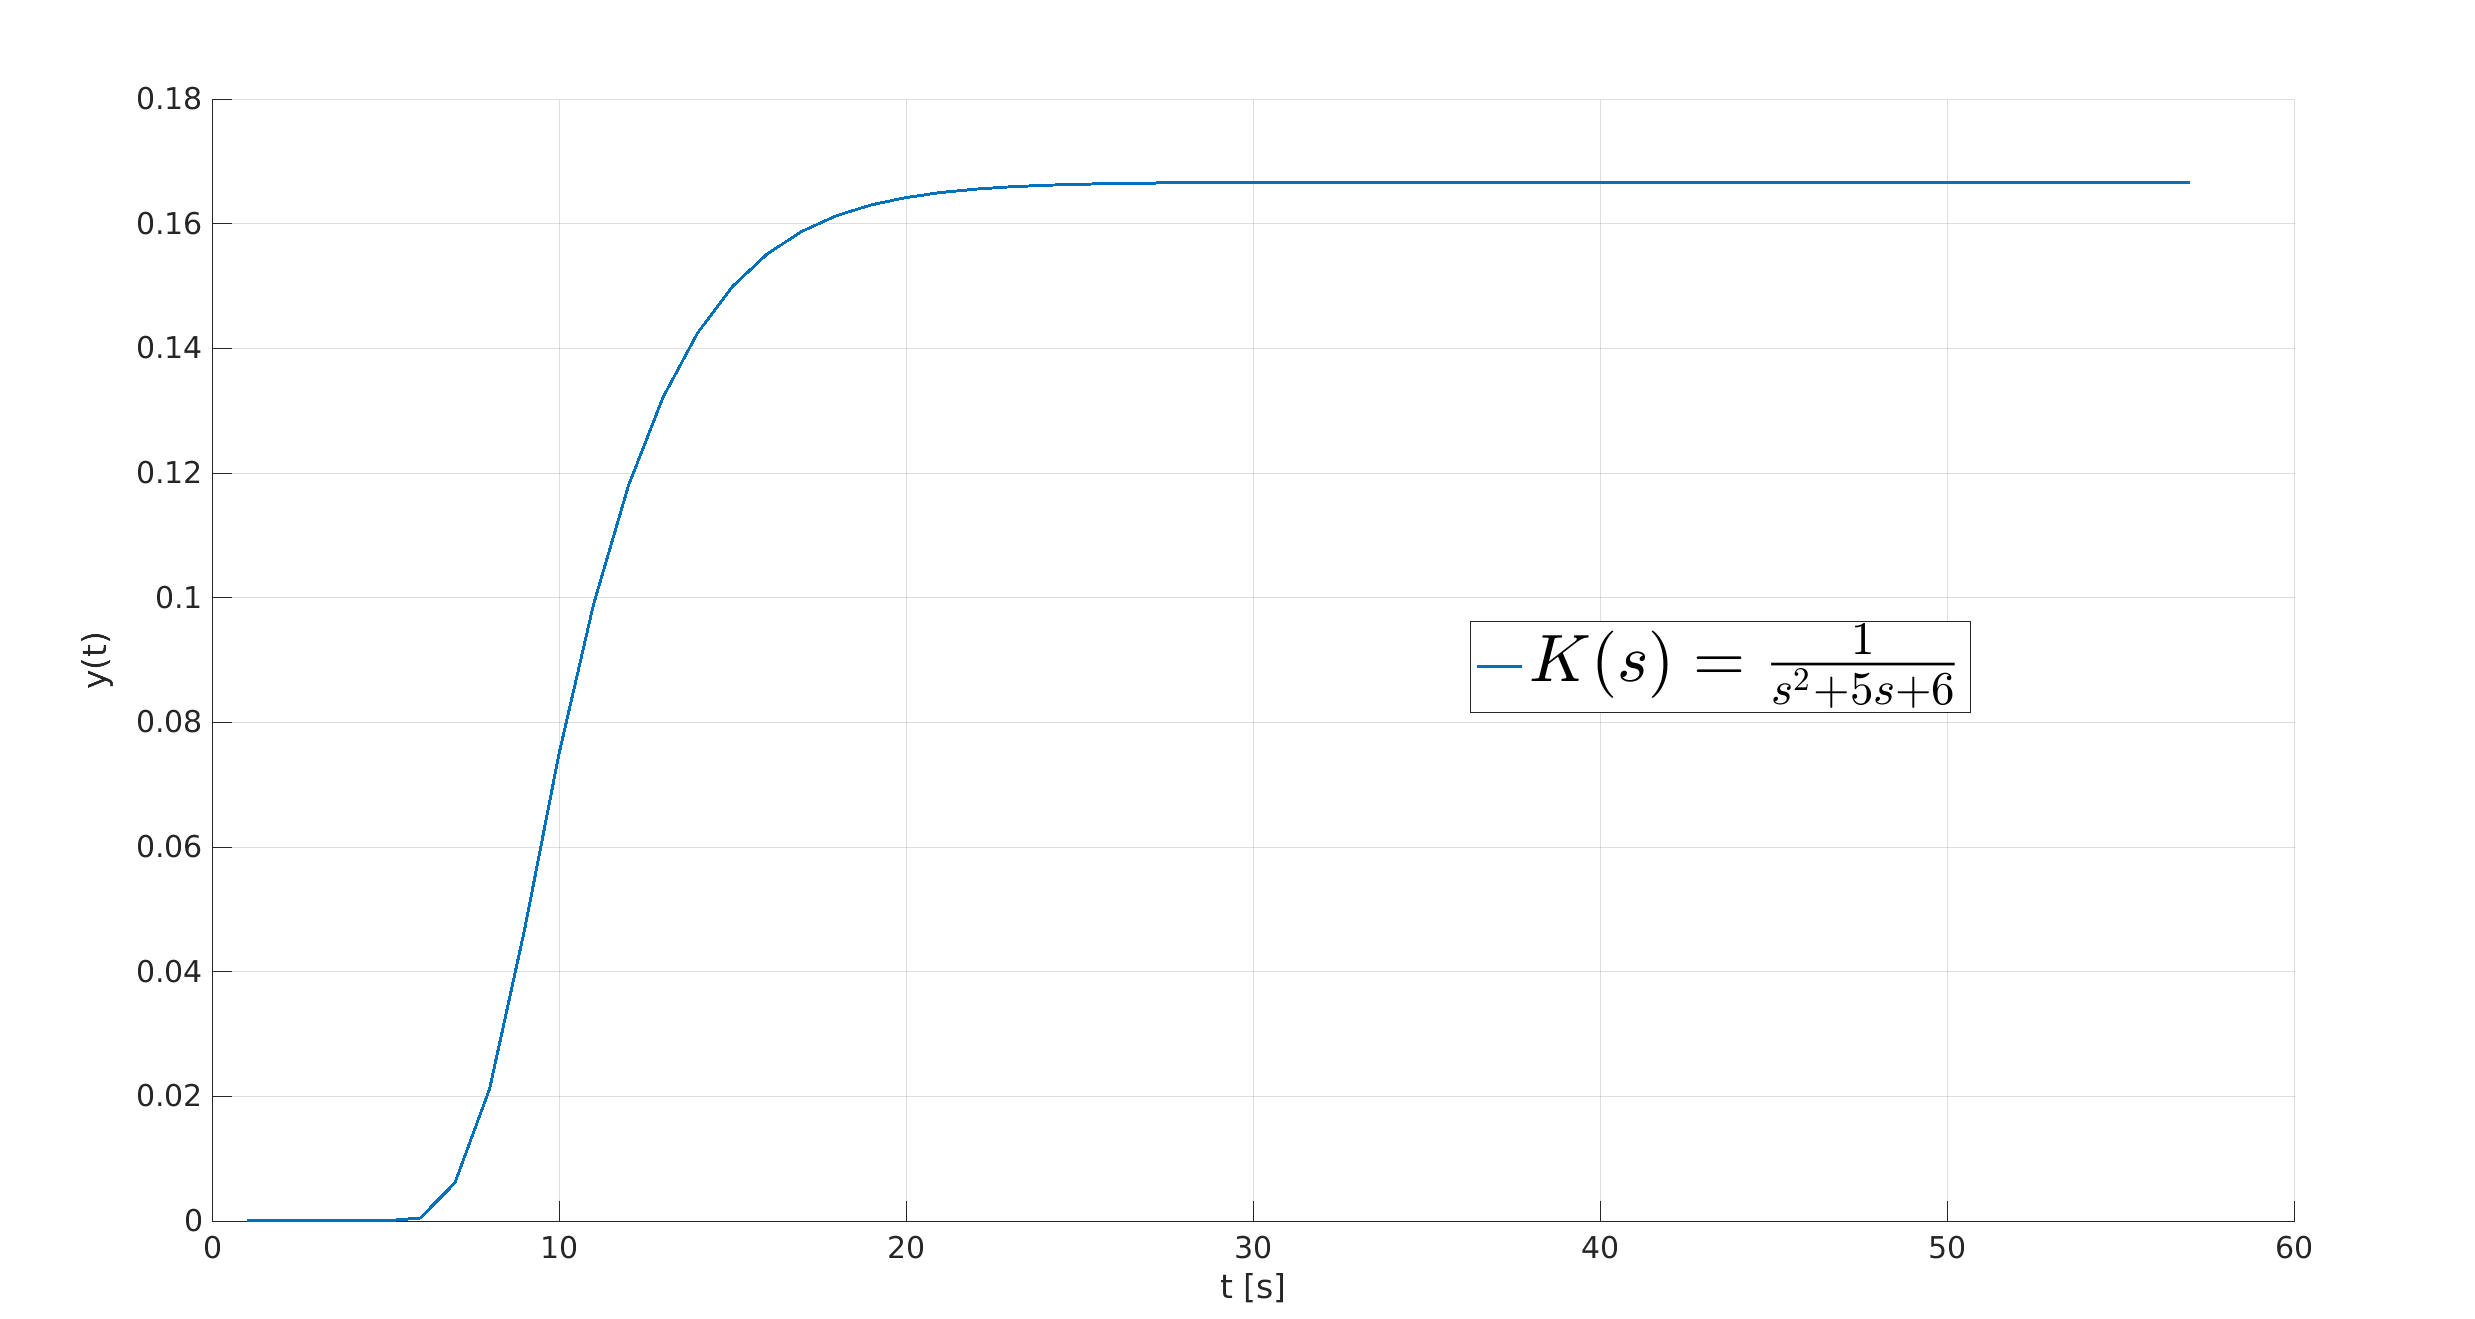
\includegraphics[width=18cm]{rzeczywiste_ujemne.png}
    \caption{Odpowiedź skokowa układu o transmitancji, której obydwa bieguny są rzeczywiste i ujemne}
\end{figure}


Układ jest stabilny (stabilizuje się na wartości $\approx 0,16667$) oraz nie ma oscylacji.


\subsubsection{Bieguny rzeczywiste o przeciwnych znakach}

Przyjmując wartości biegunów:
\begin{equation*}
    \left\{{{b_1 = -1}\atop {b_2 = 2}}\right.
\end{equation*}

Transmitancja systemu to:
\begin{equation}
    K(s) = \frac{1}{(s-(-1))(s-(2))} = \frac{1}{(s+1)(s-2)} = \frac{1}{s^2-s-2}
\end{equation}

Wygenerowano odpowiedź skokową systemu:

\begin{figure}[H]
    \centering
    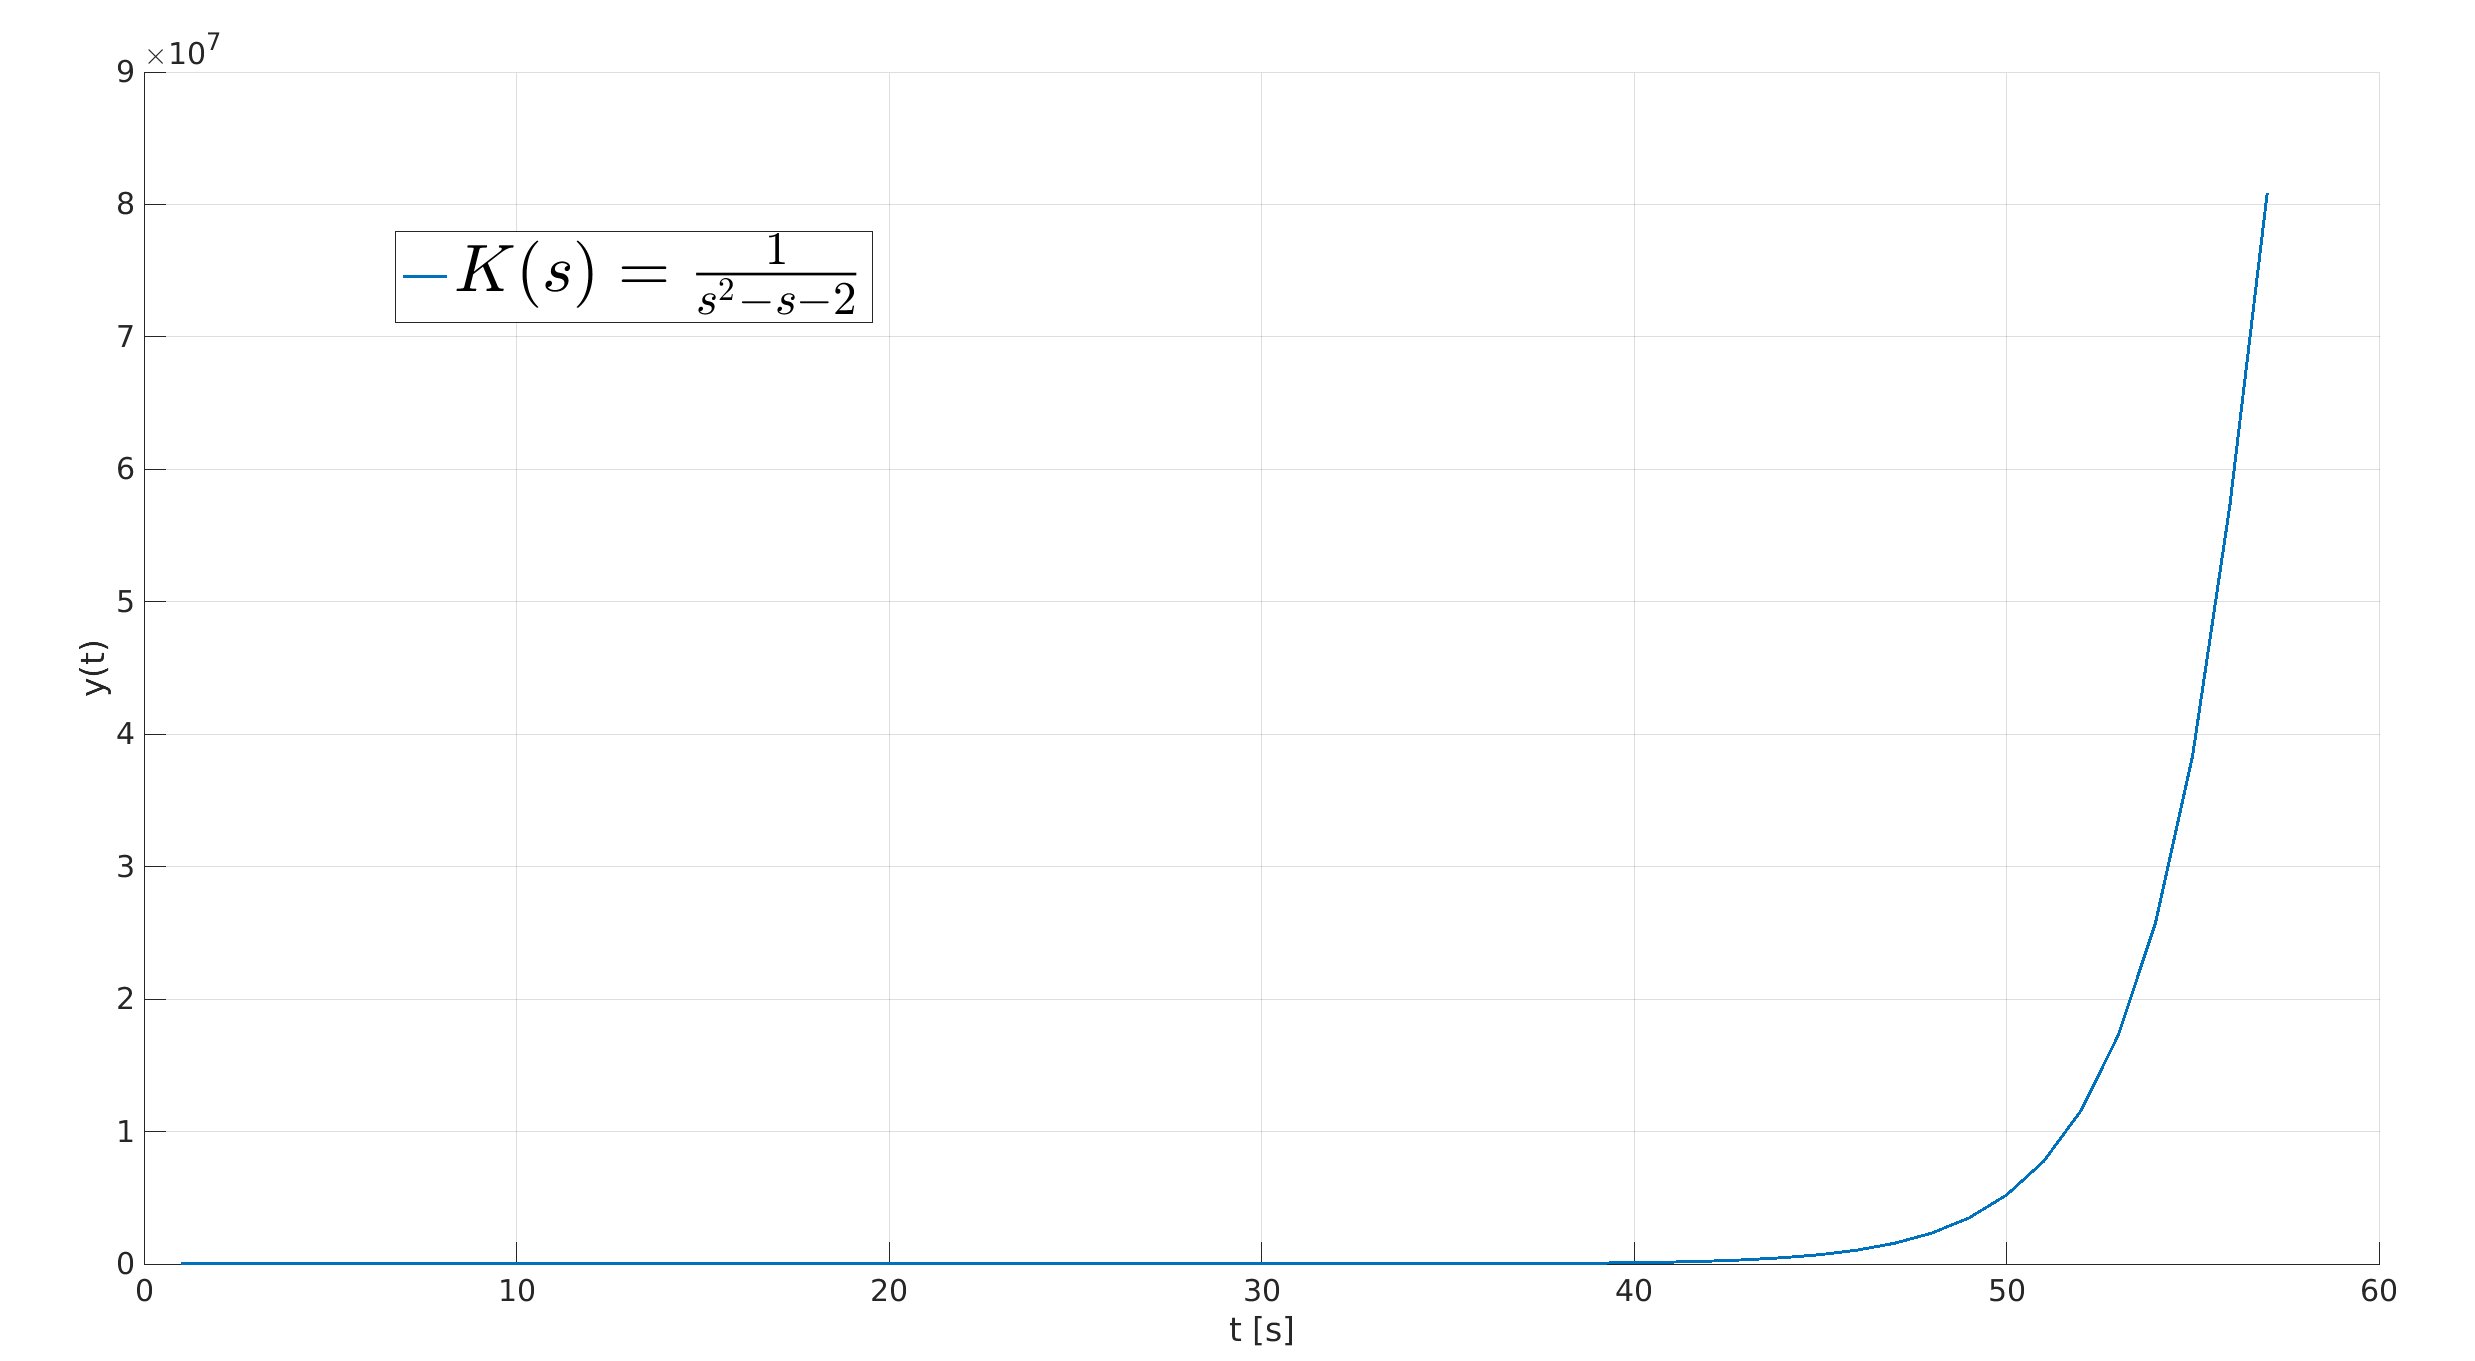
\includegraphics[width=18cm]{rzeczywiste_przeciwne_znaki.png}
    \caption{Odpowiedź skokowa układu o transmitancji, której bieguny mają przeciwne znaki}
\end{figure}

Układ nie jest stabilny oraz nie ma oscylacji.


\subsubsection{Bieguny zespolone z ujemną częścią rzeczywistą}

Przyjmując wartości biegunów:
\begin{equation*}
    \left\{{{b_1 = \frac{-0,1 + j \sqrt{3,99}}{2}}\atop {b_2 = \frac{-0,1 - j \sqrt{3,99}}{2}}}\right.
\end{equation*}

Transmitancja systemu to:
\begin{equation}
    K(s) = \frac{1}{(s-(\frac{-0,1 - j \sqrt{3,99}}{2}))(s-(\frac{-0,1 - j \sqrt{3,99}}{2}))} = \frac{1}{s^2+0,1s+1}
\end{equation}

Wygenerowano odpowiedź skokową systemu:

\begin{figure}[H]
    \centering
    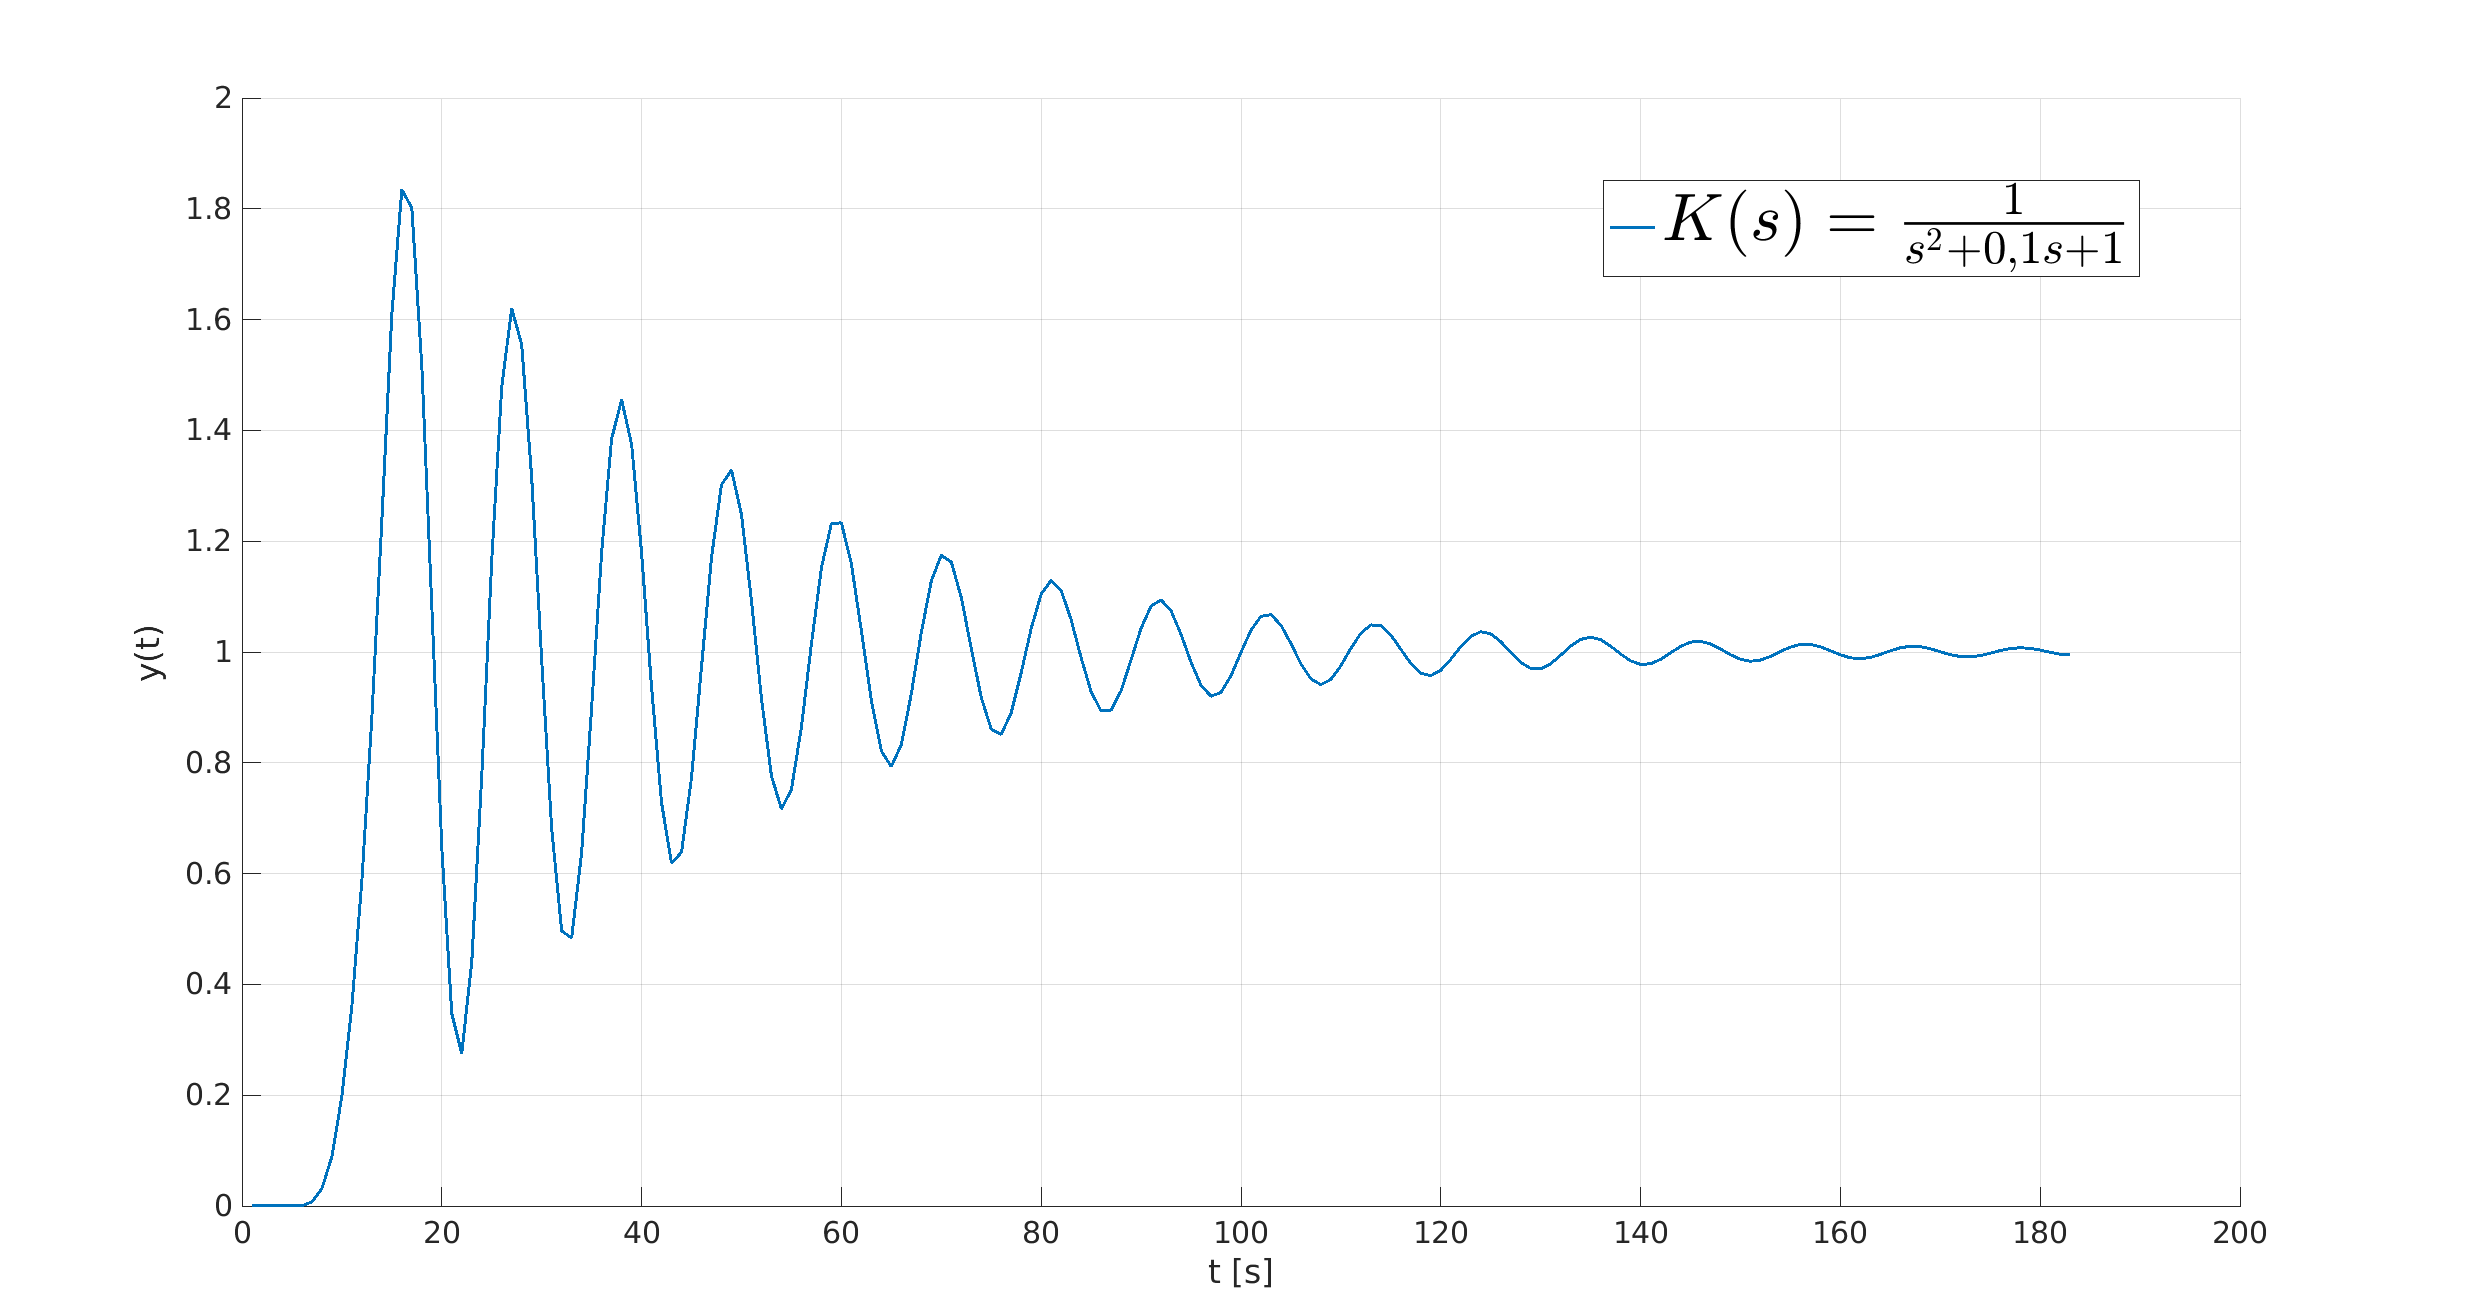
\includegraphics[width=18cm]{zespolone_ujemne.png}
    \caption{Odpowiedź skokowa układu o transmitancji, której bieguny są zespolone z ujemną częścią rzeczywistą}
\end{figure}

Układ jest stabilny (stabilizuje się na wartości $\approx 1$) oraz ma oscylacje.

\subsubsection{Bieguny zespolone z dodatnią częścią rzeczywistą}

Przyjmując wartości biegunów:
\begin{equation*}
    \left\{{{b_1 = \frac{0,1 + j \sqrt{3,99}}{2}}\atop {b_2 = \frac{0,1 - j \sqrt{3,99}}{2}}}\right.
\end{equation*}

Transmitancja systemu to:
\begin{equation}
    K(s) = \frac{1}{(s-(\frac{0,1 - j \sqrt{3,99}}{2}))(s-(\frac{0,1 - j \sqrt{3,99}}{2}))} = \frac{1}{s^2-0,1s+1}
\end{equation}

Wygenerowano odpowiedź skokową systemu:

\begin{figure}[H]
    \centering
    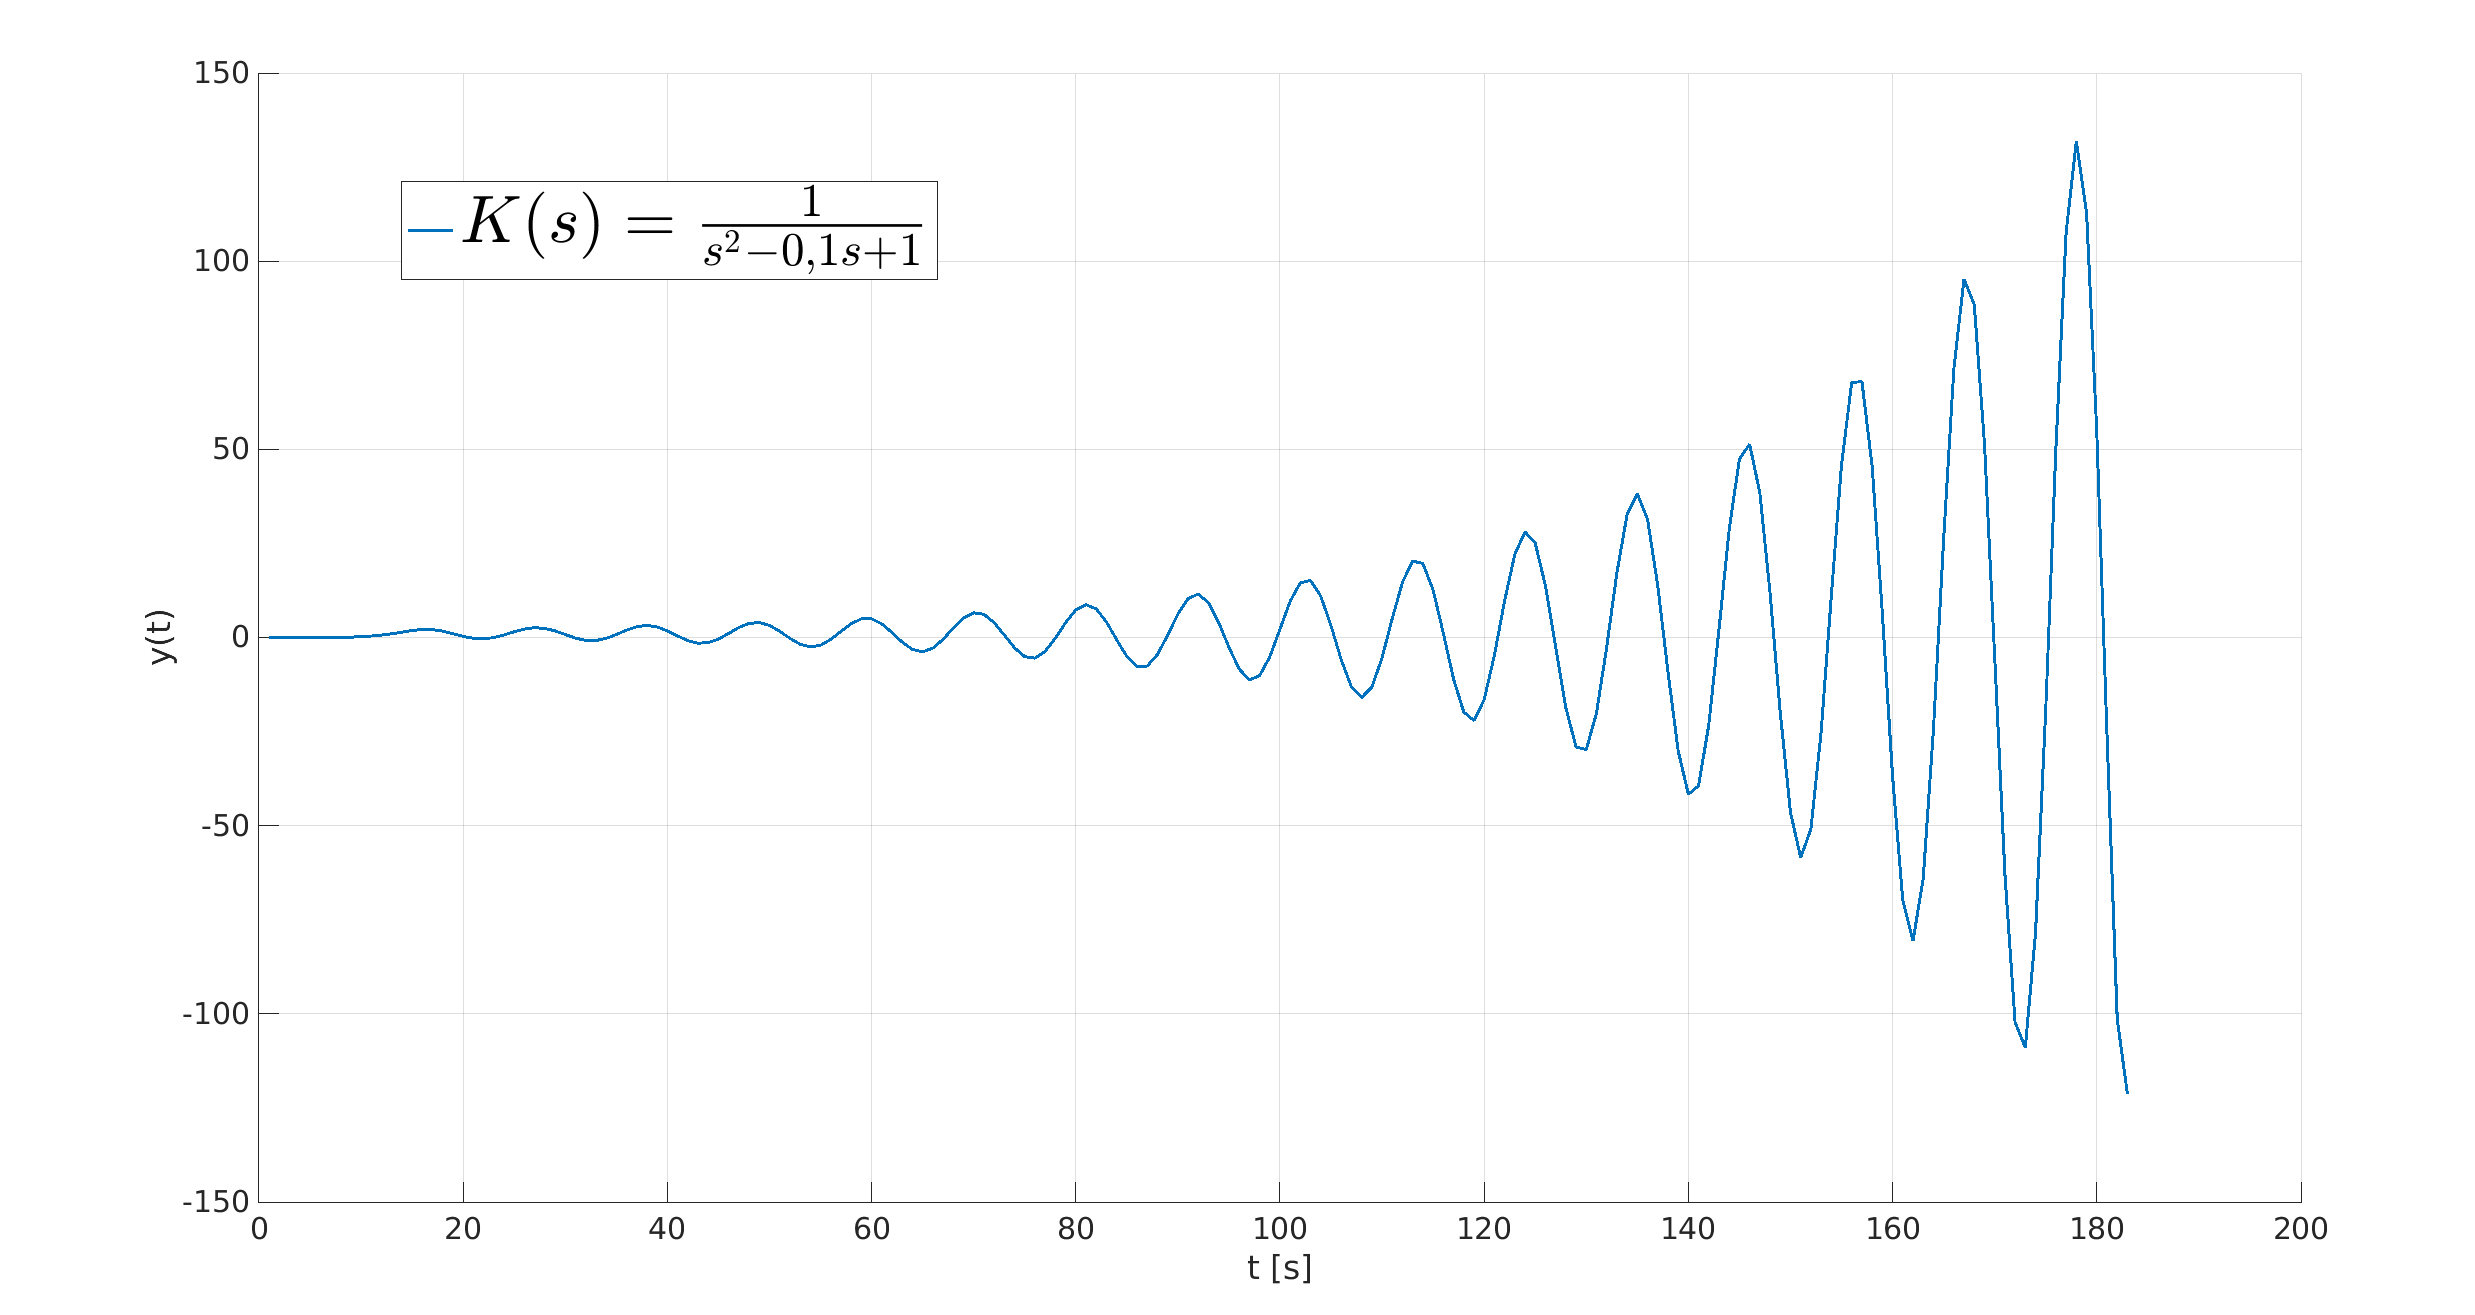
\includegraphics[width=18cm]{zespolone_dodatnia.png}
    \caption{Odpowiedź skokowa układu o transmitancji, której bieguny są zespolone z dodatnią częścią rzeczywistą}
\end{figure}

Układ nie jest stabilny oraz ma oscylacje.


\subsection{Identyfikacja systemu z czasem ciągłym na podstawie odpowiedzi skokowej}
Dana jest charakterystyka czasowa:

\begin{figure}[H]
    \centering
    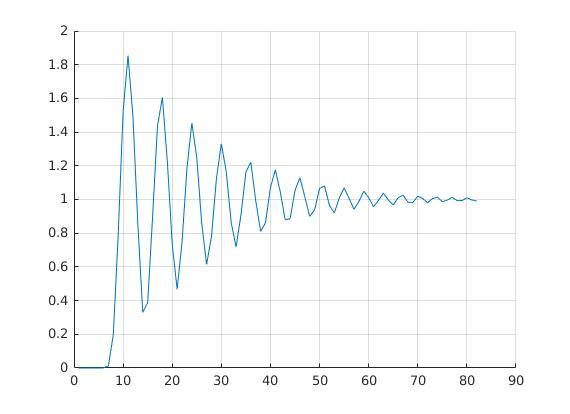
\includegraphics[width=15cm]{obojetnie.jpg}
    \caption{Odpowiedź skokowa do identyfikacji systemu}
\end{figure}

W celu identyfikacji, czyli wyznaczenia transmitancji systemu na podstawie charakterystyki czasowej, skorzystano z narzędzia dostępnego w Matlabie - \textit{Curve Fitting}. Na początku wyznaczono punkty - szczyty funkcji odpowiedzi skokowej:

\begin{figure}[H]
    \centering
    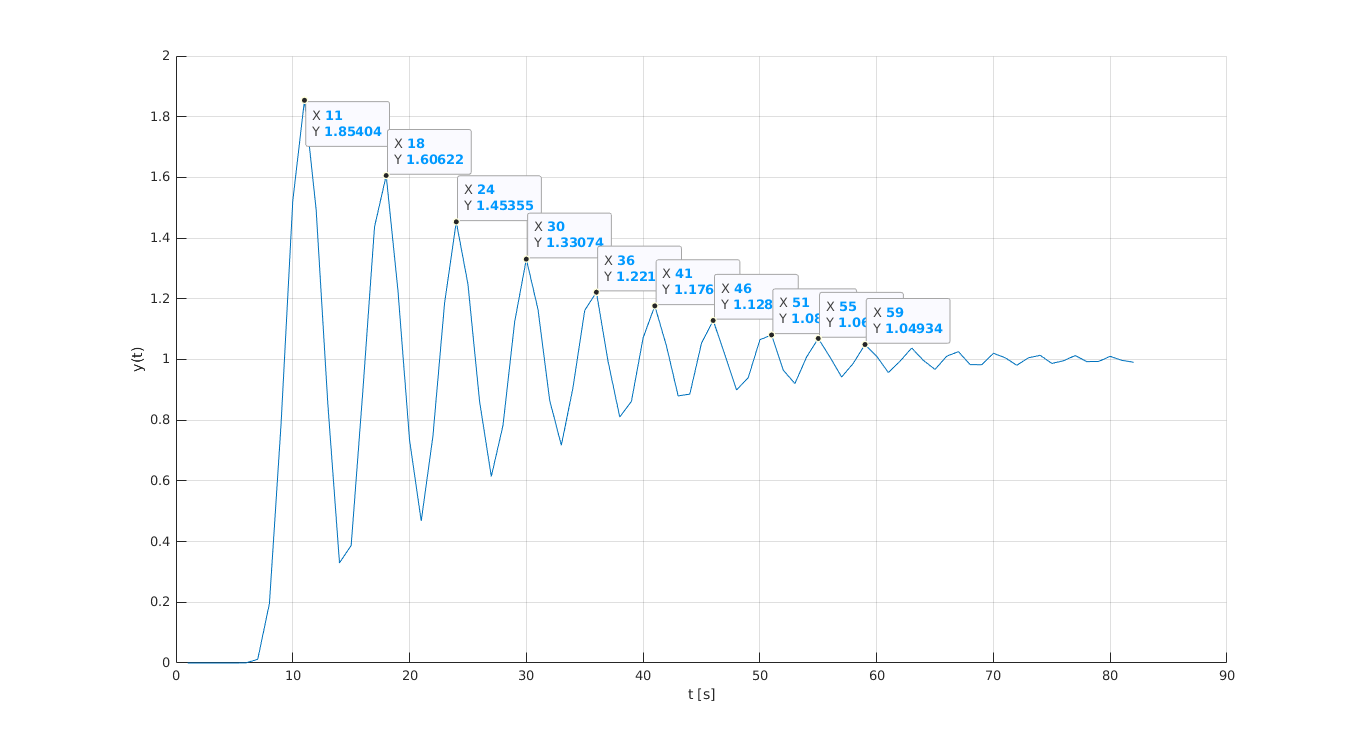
\includegraphics[width=18cm]{punkty.png}
    \caption{Punkty do wyznaczenia eksponenty}
\end{figure}

Następnie dobrano do wartości tych punktów eksponentę za pomocą \textit{Curve Fitting}:

\begin{figure}[H]
    \centering
    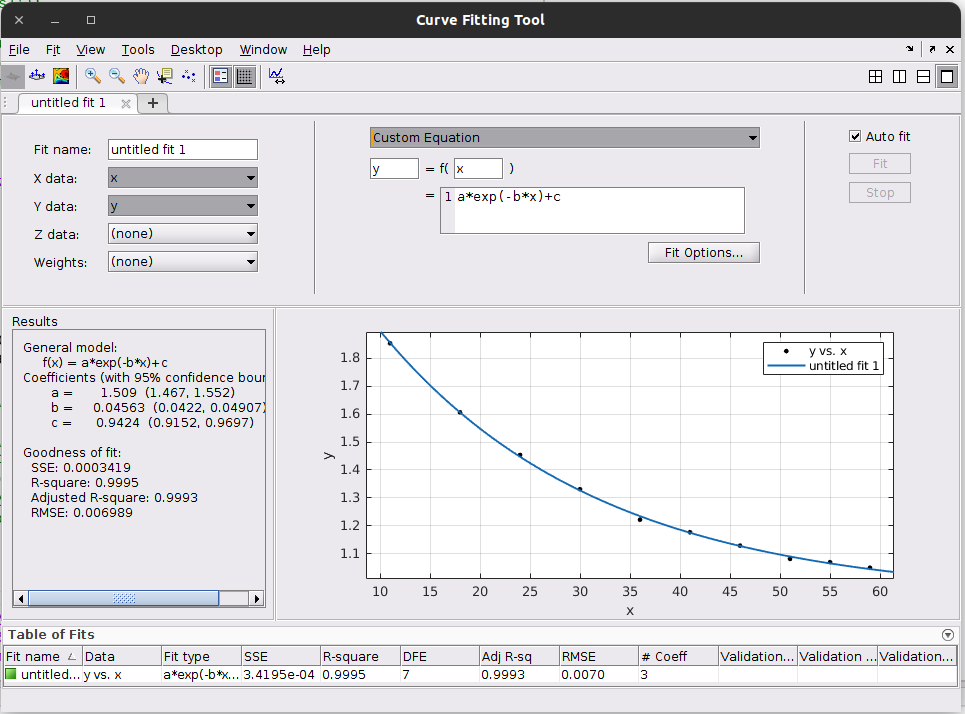
\includegraphics[width=18cm]{curve_fitting.png}
    \caption{Curve Fitting}
\end{figure}

Wzór dopasowanej przez program funkcji eksponencjalnej to:

\begin{equation}
    1,509 \cdot e^{(-0,04563x)} +0,9424
\end{equation}

Na poniższym rysunku przedstawiono odpowiedź skokową do identyfikacji wraz z dopasowaną eksponentą:

\begin{figure}[H]
    \centering
    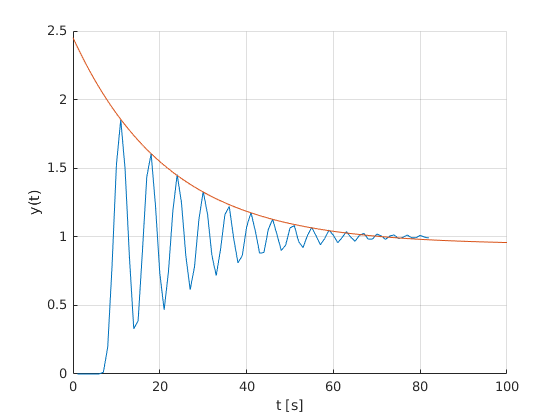
\includegraphics[width=12cm]{curve.png}
    \caption{Odpowiedź skokowa i wyznaczona eksponenta}
\end{figure}

Ze wzoru na funkcję eksponencjalną można odczytać parametry transmitancji systemu. Szukana transmitancja jest postaci:
\begin{equation}
        K(s) = \frac{1}{s^2+as+b}
\end{equation}

Z twierdzenia Abela wynika, że system ustabilizuje się na wartości, którą można wyliczyć jako granicę przy $s$ dążącym do 0. Ponadto z wykresu można odczytać, że wykres stabilizuje się na wartości 1. Zatem:

\begin{equation*}
    \lim_{s \to 0} K(s) = \frac{1}{b} = 1 \Longrightarrow b =1
\end{equation*}

Wyznaczenie parametru $a$ zaczęto od odczytania okresu oscylacji charakterystyki czasowej $T \approx 5 s$. Następnie wykorzystano poniższy wzór i wyznaczono pulsację:

\begin{equation*}
    \omega = \frac{2 \pi}{T} = \frac{2 \pi}{5} \approx 1,26
\end{equation*}

Bieguny transmitancji mają postać:

\begin{equation}
    b_{1,2} = \sigma \pm \omega j
\end{equation}

gdzie $\sigma = -0,04563 \approx -0,046$ ze wzoru eksponenty. Zatem:

\begin{equation}
    b_{1,2} = -0,046 \pm 1,26j
\end{equation}

Wstawiając wartości biegunów do transmitancji otrzymano:

\begin{equation}
    K(s) = \frac{1}{(s- (-0,046 - 1,26j))(s+0.046 + 1,26j)} = \frac{1}{s^2+0,092s+1,5876}
\end{equation}

Zatem wartość parametru $a = 0,092$.

Z identyfikacji systemu wyznaczono transmitancję:
\begin{equation}
    K(s) = \frac{1}{s^2+0,092s+1}
\end{equation}

Rzeczywista transmitancja identyfikowanego systemu miała postać:

\begin{equation}
    K(s) = \frac{1}{s^2+0,1s+1}
\end{equation}

\section{Podsumowanie i wnioski}
\begin{itemize}
    \item Zbadane zostały charakterystyki czasowe systemów w czasie ciągłym. Położenie biegunów transmitancji ma wpływ na odpowiedź skokową układu. 
    \item Bieguny rzeczywiste ujemne generują odpowiedź bez oscylacji, dążącą do pewnej stabilnej wartości. 
    \item Układ, którego bieguny są rzeczywiste, ale o przeciwnych znakach, jest niestabilny i bez oscylacji. Jego odpowiedź skokowa dąży do nieskończoności. 
    \item Układ z biegunami zespolonymi z ujemną częścią rzeczywistą generuje odpowiedź skokową z gasnącymi oscylacjami. Taki układ jest stabilny. 
    \item Bieguny zespolone z dodatnią częścią rzeczywistą generują odpowiedź skokową, której oscylacje narastają. Układ jest niestabilny.
    \item Matlab posiada narzędzia, które umożliwiają identyfikację systemu (Curve Fitting).
    \item Transmitancja wyznaczona eksperymentalnie na podstawie odpowiedzi skokowej w przybliżeniu zgadza się z transmitancją rzeczywistą. Różnica przy parametrze $a$ to $0,08$.
\end{itemize}

\section{Bibliografia}
\begin{enumerate}
    \item A. Czemplik "Praktyczne wprowadzenie do opisu, analizy i symulacji dynamiki obiektów"
    \item K. Duzinkiewicz, Prezentacja "Obiekty sterowania i ich identyfikacja", Komputerowe systemy sterowania 2014/2015 
\end{enumerate}

\end{document}